\documentclass[11pt]{amsart}

\usepackage[margin=1.1in]{geometry}
\usepackage{amsmath,amssymb,amsthm}
\usepackage{booktabs}
\usepackage{graphicx}
\usepackage[numbers,sort&compress]{natbib}
\usepackage[hidelinks]{hyperref}

\newtheorem{theorem}{Theorem}[section]
\newtheorem{proposition}[theorem]{Proposition}
\newtheorem{lemma}[theorem]{Lemma}
\newtheorem{corollary}[theorem]{Corollary}
\theoremstyle{definition}
\newtheorem{definition}[theorem]{Definition}
\theoremstyle{remark}
\newtheorem{remark}[theorem]{Remark}

\newcommand{\R}{\mathbb{R}}
\newcommand{\tr}{\operatorname{tr}}
\newcommand{\T}{^{\top}}
\newcommand{\Ib}{I(z)}

\title[Exchange-stable D-optimal binning of scores]{Exchange-stable D-optimal partitions of score
vectors are nearest-centroid rules}
\author{Vitaly Vorobyev}
\date{October 2026}
\subjclass[2020]{Primary 62K05; Secondary 62B10, 62H30, 94A29}
\keywords{Fisher information, quantization, D-optimality, exchange algorithm, Voronoi partition,
nuisance parameters, formal verification}


\begin{document}

\begin{abstract}
Hard binning of events before a likelihood fit keeps the Fisher information of the bin labels
and loses the rest. For a finite weighted sample of score vectors and a labelling~$z$ into
$K$ cells, the retained information is $\Ib=\sum_c W_c\mu_c\mu_c\T$, where $W_c$ is the mass
and $\mu_c$ the mean score of cell~$c$. We study the D-optimal problem of maximizing
$\log\det\Ib$. We prove that if duplicate scores are merged, the weights are positive, every cell
is nonempty and $\Ib$ is nonsingular, then every labelling that no single-point move can
improve is strictly nearest-centroid in the metric $\Ib^{-1}$. The nearest-centroid rule built
from such a labelling therefore reproduces it exactly. For a scalar parameter this reduces to
known facts about score-function quantizers and Hartigan's $k$-means method; the content is the
determinant criterion for a vector parameter. The proof is machine-checked in Lean~4 with
Mathlib. We also give exact examples showing that the iteration ``assign to the nearest centroid
in the current metric'' can decrease the objective, that a strict nearest-centroid labelling need
not be stable, and that a global optimum of the profiled $D_s$ criterion can violate the
nearest-centroid rule of its own efficient metric.
\end{abstract}

\maketitle

\section{Introduction}\label{sec:intro}

Many analyses replace each observation by one of $K$ bin labels before estimating a parameter
$\theta\in\R^d$: histograms in particle physics, gates in cytometry, quantized measurements in
sensor networks. The labels are only as useful as the Fisher information they keep. At a
reference point $\theta_0$ the natural representation of an observation $x$ for this purpose is
its score $s=\nabla_\theta\log p(x\mid\theta)|_{\theta_0}$, because the information carried by a
label $Z$ is the covariance of $\mathbb{E}[S\mid Z]$, which is fixed by how the label groups
scores~\cite{venkitasubramaniam2006,barnes2020}. Binning for estimation is then a problem of partitioning
score space.

For a scalar parameter the problem is well understood. Quantizers that threshold the score are
optimal for the Fisher information at a fixed parameter value~\cite{venkitasubramaniam2006,venkitasubramaniam2007}, and on a finite
sample the problem is $k$-means on the scalar score (Section~\ref{sec:setting}). For a vector
parameter one must choose a matrix criterion. Maximizing the trace of the retained information is
again $k$-means, now on the vector scores, and for exponential families some optimal partition
of this kind has convex polyhedral cells~\cite{dulek2023}. This paper is about the D criterion, $\log\det$ of the retained
information, which is invariant under reparametrization and is the usual choice when all
components of $\theta$ matter~\cite{karlin1966}.

The tool is single-point exchange: move one observation to another cell if that raises the
objective. Its exact determinant update is classical
\cite{banfield1977,fedorov1972,mitchell1974,cook1980}, and for $k$-means it is known that every
labelling stable under such moves is a Voronoi partition, while the converse
fails~\cite{telgarsky2010}. We prove the analogue for the D criterion:

\begin{quote}
\emph{every exchange-stable labelling is strictly nearest-centroid in the metric $\Ib^{-1}$,
where $\Ib$ is the information of the labelling itself}
\end{quote}
(Theorem~\ref{thm:main}, with all hypotheses stated there). The metric depends on the partition,
and the criterion is not a separable sum over cells, so neither the $k$-means argument nor the
partition theorem of Barnes, Hoffman and Rothblum~\cite{barnes1992} applies
(Section~\ref{sec:related}). The consequence that matters in practice is that a stable labelling
of a training sample defines a rule for new observations, the nearest centroid in $\Ib^{-1}$,
and that this rule reproduces the training labels without any tie-breaking convention
(Corollary~\ref{cor:compile}).

The contribution is modest and structural. It is not a new algorithm: the exchange algorithm and
its update formulas are known, and we credit them in Section~\ref{sec:moves}. What we add is the
theorem, its machine-checked proof, and exact examples marking where it stops. Two of them are
new for the D criterion: the batch nearest-centroid iteration can decrease the objective, and
with nuisance parameters profiled out even a global optimum can violate the nearest-centroid
rule of its own efficient metric. Two others are one-dimensional, where D coincides with
$k$-means, and restate known facts: a strict nearest-centroid labelling need not be
stable~\cite{telgarsky2010}, and unmerged duplicate scores break the conclusion. They are
included to show that the hypotheses of the theorem are needed.

\section{Setting}\label{sec:setting}

\subsection*{The weighted sample and its partitions}
A sample is a list of score vectors $s_1,\dots,s_N\in\R^d$ with weights $w_1,\dots,w_N>0$. A
labelling is a map $z:\{1,\dots,N\}\to\{1,\dots,K\}$. For a cell $c$ write $C_c=\{i:z_i=c\}$ and
\[
W_c=\sum_{i\in C_c}w_i,\qquad m_c=\sum_{i\in C_c}w_is_i,\qquad \mu_c=m_c/W_c .
\]
Throughout, every cell is nonempty, so $W_c>0$ and the centroid $\mu_c$ is defined. The
retained information of $z$ is
\begin{equation}\label{eq:info}
\Ib=\sum_{c=1}^K W_c\,\mu_c\mu_c\T=\sum_{c=1}^K \frac{m_cm_c\T}{W_c}.
\end{equation}
It is positive semidefinite, and positive definite exactly when it is nonsingular.

\subsection*{What $\Ib$ means}
Let $T=\sum_i w_is_is_i\T$. A direct expansion gives the identity
\begin{equation}\label{eq:pythagoras}
T-\Ib=V(z),\qquad V(z)=\sum_{c}\sum_{i\in C_c}w_i(s_i-\mu_c)(s_i-\mu_c)\T\succeq0 .
\end{equation}
If the weighted sample is the law of the score $S$ at $\theta_0$, or a Monte Carlo
approximation of it, with $\mathbb{E}S=0$, then $T$ is (an estimate of) the Fisher information of
the observation and $\Ib$ that of the bin label $Z$, namely $\operatorname{Var}\mathbb{E}[S\mid Z]$
\cite{venkitasubramaniam2006,barnes2018,barnes2020}. Identity~\eqref{eq:pythagoras} then says that
binning loses exactly the score variation within cells. None of the results below uses
$\mathbb{E}S=0$; they are statements about the finite object~\eqref{eq:info}. When the scores are
centred, $\sum_cm_c=0$ and $\operatorname{rank}\Ib\le K-1$, so a nonsingular $\Ib$ needs
$K\ge d+1$ cells.

When $T\succ0$, the eigenvalues of $T^{-1/2}\Ib\,T^{-1/2}$ lie in $[0,1]$
by~\eqref{eq:pythagoras}, and $(\det\Ib/\det T)^{1/d}$ is the usual D-efficiency of the binning.
We call it the retention.

\subsection*{The D criterion}
The D-optimal binning problem is
\begin{equation}\label{eq:dopt}
\max_{z}\ \log\det\Ib\quad\text{over labellings with $K$ nonempty cells.}
\end{equation}
By~\eqref{eq:pythagoras} this is $\max\det(T-V(z))$. Three neighbouring criteria are useful
landmarks: $\max\tr\Ib$ is $\min\tr V(z)$, which is $k$-means on the scores; Friedman and
Rubin's $\min\det V(z)$~\cite{friedman1967,marriott1971,scott1971} is a classical clustering
criterion; and $\max\det(T-V(z))$ is neither. For $d=1$ all three coincide with $k$-means on the
scalar score, so anything new lives in $d\ge2$. Under an invertible reparametrization
$\theta=A\phi$ the scores become $A\T s$ and $\Ib$ becomes $A\T\Ib A$. This multiplies
$\det\Ib$ by $\det(A)^2$, so it adds the constant $2\log|\det A|$ to the objective, and it leaves the metric $(s-\mu)\T\Ib^{-1}(s-\mu)$ unchanged, so both the
D-optimal partitions and the geometry below do not depend on the coordinates of~$\theta$.

\section{Exact single-point moves}\label{sec:moves}

\begin{definition}\label{def:move}
A relocation of row $i$ from its cell $a=z_i$ to a cell $b\ne a$ is \emph{admissible} if $C_a$
contains some row other than $i$, so that no cell is emptied. Write $z^{i\to b}$ for the
relocated labelling. A labelling $z$ is \emph{exchange stable} if
$\det I(z^{i\to b})\le\det\Ib$ for every admissible relocation.
\end{definition}

For an admissible move of row $i$, with $s=s_i$ and $w=w_i$, put
\begin{equation}\label{eq:coeffs}
u_a=\mu_a-s,\quad u_b=\mu_b-s,\qquad \alpha=\frac{wW_a}{W_a-w},\qquad \beta=\frac{wW_b}{W_b+w}.
\end{equation}
Since $W_a>w>0$ and $W_b>0$, both coefficients are positive, and $\beta<w<\alpha$.

\begin{proposition}[rank-two update]\label{prop:rank2}
For an admissible relocation of row $i$ from $a$ to a nonempty cell $b$,
\[
I(z^{i\to b})-\Ib=\alpha\,u_au_a\T-\beta\,u_bu_b\T .
\]
\end{proposition}

\begin{proof}
Only cells $a$ and $b$ change. In cell $a$, write $m_a'=m_a-ws=(W_a-w)\mu_a+wu_a$. Expanding
$m_a'm_a'^{\top}/(W_a-w)-W_a\mu_a\mu_a\T$ and using $\mu_a-u_a=s$ gives
$-wss\T+\alpha u_au_a\T$. The same computation for cell $b$, with $m_b'=(W_b+w)\mu_b-wu_b$,
gives $wss\T-\beta u_bu_b\T$. The $ss\T$ terms cancel.
\end{proof}

\begin{proposition}[determinant ratio]\label{prop:detratio}
Let $I\in\R^{d\times d}$ be symmetric and nonsingular, $G=I^{-1}$, $\alpha,\beta\in\R$ and
$u_a,u_b\in\R^d$. With $q_{aa}=u_a\T Gu_a$, $q_{bb}=u_b\T Gu_b$ and $q_{ab}=u_a\T Gu_b$,
\begin{equation}\label{eq:ratio}
\det\bigl(I+\alpha u_au_a\T-\beta u_bu_b\T\bigr)=\det I\cdot\rho,\qquad
\rho=(1+\alpha q_{aa})(1-\beta q_{bb})+\alpha\beta q_{ab}^2 .
\end{equation}
If moreover $\det I>0$ and $\rho>0$, the change of $\log\det$ is $\log\rho$.
\end{proposition}

\begin{proof}
Write the update as $UCU\T$ with $U=[u_a\;u_b]$ and $C=\operatorname{diag}(\alpha,-\beta)$. By
the Weinstein--Aronszajn identity, $\det(I+UCU\T)=\det I\cdot\det(\mathrm{Id}_2+CU\T GU)$, and the
$2\times2$ determinant is $\rho$ because $G$ is symmetric, so $u_b\T Gu_a=q_{ab}$.
\end{proof}

Both propositions are known in substance. Banfield and Bassill's transfer algorithm for
$\min\det V$~\cite{banfield1977} uses exactly this rank-two change of the within-cell scatter
and its determinant ratio; since $\Ib=T-V(z)$ with $T$ fixed, the same algebra applies here
verbatim. Exchange algorithms for exact D-optimal designs rest on the same determinant-lemma
updates~\cite{fedorov1972,mitchell1974,cook1980}. With $G$ cached, a candidate move costs $O(d^2)$,
and an accepted move updates $G$ by the Woodbury identity. We write
\[
\kappa=\rho-1=\alpha q_{aa}-\beta q_{bb}-\alpha\beta\,(q_{aa}q_{bb}-q_{ab}^2)
\]
for the excess of the ratio over one.

\section{Exchange stability forces nearest-centroid geometry}\label{sec:main}

\noindent\textbf{Standing hypotheses (H).} The scores $s_1,\dots,s_N$ are pairwise distinct
(duplicates have been merged, Proposition~\ref{prop:merge}); the weights are positive; all $K$
cells of $z$ are nonempty; and $\Ib$ is nonsingular. We write $G=\Ib^{-1}$ and
$\|v\|_G^2=v\T Gv$.

\begin{lemma}[leverage]\label{lem:leverage}
If every cell is nonempty and $\Ib\succ0$, then for all cells $c$ and $a,b$,
\[
\mu_c\T G\mu_c\le\frac1{W_c},\qquad (\mu_a-\mu_b)\T G(\mu_a-\mu_b)\le\frac1{W_a}+\frac1{W_b}.
\]
\end{lemma}

\begin{proof}
Let $A\in\R^{d\times K}$ have columns $\sqrt{W_c}\,\mu_c$, so $\Ib=AA\T$. Then
$P=A\T(AA\T)^{-1}A$ is symmetric and idempotent, hence $v\T Pv\le v\T v$ for every
$v\in\R^K$. Taking $v=e_c/\sqrt{W_c}$ gives the first bound; taking
$v=e_a/\sqrt{W_a}-e_b/\sqrt{W_b}$, for which $Av=\mu_a-\mu_b$, gives the second.
\end{proof}

\begin{lemma}[scalar core]\label{lem:scalar}
Let $0<w<W_a$, $W_b>0$, and $\alpha,\beta$ as in~\eqref{eq:coeffs}. Let $q_{aa},q_{bb},q_{ab}$
be real numbers with $0\le q_{bb}\le q_{aa}$, and put $q_\delta=q_{aa}+q_{bb}-2q_{ab}$. If
$0\le q_\delta\le 1/W_a+1/W_b$, then
\[
\kappa\ \ge\ \frac{\alpha\beta}{4}\Bigl(q_\delta^2+(q_{aa}-q_{bb})^2\Bigr).
\]
\end{lemma}

\begin{proof}
From $1/\alpha=1/w-1/W_a$ and $1/\beta=1/w+1/W_b$ we get
$\alpha-\beta=\alpha\beta\,(1/W_a+1/W_b)$, so the hypothesis on $q_\delta$ gives
$\alpha-\beta-\alpha\beta q_\delta\ge0$. Substituting $q_{ab}=(q_{aa}+q_{bb}-q_\delta)/2$ into
$\kappa$ and expanding gives the identity
\[
\kappa=\frac{\alpha\beta}{4}\Bigl(q_\delta^2+(q_{aa}-q_{bb})^2\Bigr)
+\tfrac12\bigl(\alpha-\beta-\alpha\beta q_\delta\bigr)(q_{aa}+q_{bb})
+\tfrac12(\alpha+\beta)(q_{aa}-q_{bb}),
\]
whose last two terms are nonnegative.
\end{proof}

\begin{proposition}[gain of a violating move]\label{prop:gain}
Assume (H), and let the relocation of row $i$ from $a=z_i$ to $b$ be admissible. If $s_i$ is at
least as close to $\mu_b$ as to its own centroid,
$\|s_i-\mu_b\|_G\le\|s_i-\mu_a\|_G$, then
\[
\det I(z^{i\to b})\ \ge\ \det\Ib\Bigl(1+\frac{\alpha\beta}{4}\,q_\delta^2\Bigr),\qquad
q_\delta=\|\mu_a-\mu_b\|_G^2 .
\]
If in addition $\mu_a\ne\mu_b$, then $\log\det I(z^{i\to b})-\log\det\Ib\ge
\log(1+\alpha\beta q_\delta^2/4)>0$.
\end{proposition}

\begin{proof}
By Propositions~\ref{prop:rank2} and~\ref{prop:detratio}, $\det I(z^{i\to b})=\det\Ib(1+\kappa)$ with
the $q$'s of~\eqref{eq:ratio} formed from $u_a,u_b$ and $G$. Since $G\succ0$, $q_{aa},q_{bb}\ge0$;
the hypothesis is $q_{bb}\le q_{aa}$; and since $u_a-u_b=\mu_a-\mu_b$ and $G$ is symmetric,
$q_{aa}+q_{bb}-2q_{ab}=q_\delta\ge0$. Lemma~\ref{lem:leverage} gives
$q_\delta\le1/W_a+1/W_b$, so Lemma~\ref{lem:scalar} applies, and $\det\Ib>0$. If
$\mu_a\ne\mu_b$ then $q_\delta>0$ because $G\succ0$.
\end{proof}

\begin{lemma}[stability separates centroids]\label{lem:distinct}
Under (H), if $z$ is exchange stable then $\mu_a\ne\mu_b$ for all cells $a\ne b$.
\end{lemma}

\begin{proof}
Suppose $\mu_a=\mu_b$ and $|C_a|\ge2$. Because the scores are distinct, at most one row of $C_a$
sits at $\mu_a$, so some $i\in C_a$ has $s_i\ne\mu_a$. Moving it to $b$ is admissible, and
$u_a=u_b=u$ with $q=u\T Gu>0$, so $\rho=(1+\alpha q)(1-\beta q)+\alpha\beta q^2=1+(\alpha-\beta)q>1$,
contradicting stability. Hence, by symmetry, $|C_a|=|C_b|=1$; but then $\mu_a$ and $\mu_b$ are two scores of
the sample, and they are distinct.
\end{proof}

\begin{theorem}[exchange stability implies strict nearest-centroid geometry]\label{thm:main}
Let $s_1,\dots,s_N\in\R^d$ be pairwise distinct with weights $w_i>0$, and let
$z:\{1,\dots,N\}\to\{1,\dots,K\}$ have all $K$ cells nonempty and $\Ib$ nonsingular. If no
admissible relocation strictly increases $\det\Ib$, then for every row $i$ and every cell
$c\ne z_i$,
\[
(s_i-\mu_{z_i})\T\,\Ib^{-1}(s_i-\mu_{z_i})\ <\ (s_i-\mu_c)\T\,\Ib^{-1}(s_i-\mu_c).
\]
\end{theorem}

\begin{proof}
Fix $i$ and $c\ne z_i=a$. By Lemma~\ref{lem:distinct}, $\mu_a\ne\mu_c$. If $|C_a|\ge2$, the move
of $i$ to $c$ is admissible, and if $s_i$ were at least as close to $\mu_c$ as to $\mu_a$,
Proposition~\ref{prop:gain} would give it a strictly positive gain, contradicting stability. If
$|C_a|=1$, then $\mu_a=s_i$, so the left side is $0$, while the right side is
$\|\mu_a-\mu_c\|_G^2>0$.
\end{proof}

Stability with respect to $\log\det$ is the same hypothesis: at a nonsingular $\Ib$, a candidate
raises $\log\det$ exactly when it raises $\det$ (a singular candidate has $\log\det=-\infty$).
Proposition~\ref{prop:gain} is quantitative: a point that prefers another centroid is worth at
least $\log(1+\alpha\beta q_\delta^2/4)$ nats to move. This is the form in which the guarantee
survives a positive gain tolerance (Section~\ref{sec:alg}).

\begin{remark}[the scalar case]
For $d=1$, $\Ib=T-V(z)$ is a number, the metric is a positive multiple of the Euclidean one, and
an admissible move changes $\Ib$ by $\alpha u_a^2-\beta u_b^2$, which is exactly the decrease of
the $k$-means cost under Hartigan's transfer. Theorem~\ref{thm:main} is then the weighted form of
the observation of Telgarsky and Vattani that partitions stable under Hartigan's method are
Voronoi partitions~\cite{telgarsky2010},
and its population counterpart is the threshold form of score-function
quantizers~\cite{venkitasubramaniam2006}. The theorem is new only for $d\ge2$.
\end{remark}

\begin{corollary}[global optima]\label{cor:global}
Let the sample be as in Theorem~\ref{thm:main}. If $z$ maximizes $\det I(z')$ over all labellings
$z':\{1,\dots,N\}\to\{1,\dots,K\}$, has all $K$ cells nonempty and $\Ib$ nonsingular, then $z$ is
strictly nearest-centroid in $\Ib^{-1}$.
\end{corollary}

\begin{proof}
A relocation is a relabelling, so a global maximizer is exchange stable.
\end{proof}

A rule $r:\R^d\to\{1,\dots,K\}$ is a \emph{nearest-centroid rule} of $z$ if
$\|s-\mu_{r(s)}\|_G\le\|s-\mu_c\|_G$ for all $s\in\R^d$ and all $c$; ties may be broken
arbitrarily, even inconsistently.

\begin{corollary}[the compiled rule reproduces the labels]\label{cor:compile}
Under the hypotheses of Theorem~\ref{thm:main}, a nearest-centroid rule exists when $d\ge1$,
and every nearest-centroid rule $r$ satisfies $r(s_i)=z_i$ for all $i$.
\end{corollary}

\begin{proof}
Existence: the minimum over finitely many cells is attained ($K\ge1$, since $K=0$ would make
$\Ib=0$ singular). Reproduction: by Theorem~\ref{thm:main} the minimum at $s_i$ is attained only
at $z_i$.
\end{proof}

Real samples contain repeated scores, from discrete observables or repeated simulation. The
theorem is applied after merging them.

\begin{proposition}[duplicates]\label{prop:merge}
Let $(s'_j,w'_j)_{j\le N'}$ be a sample with positive weights, and let
$\pi:\{1,\dots,N'\}\to\{1,\dots,N\}$ merge it into $(s_i,w_i)_{i\le N}$, that is,
$s'_j=s_{\pi(j)}$ and $w_i=\sum_{\pi(j)=i}w'_j$. For any labelling $z$ of the merged sample, the
inherited labelling $z\circ\pi$ of the original rows has the same cell masses, cell sums,
centroids and retained information as $z$. Consequently, if the merged sample and $z$ satisfy the
hypotheses of Theorem~\ref{thm:main}, then every nearest-centroid rule of the unmerged sample
labelled by $z\circ\pi$ assigns every original row the label of its atom.
\end{proposition}

\begin{proof}
Cell sums and masses are sums over the fibres of $\pi$, which regroup without change. The rule
built from the unmerged data is therefore a nearest-centroid rule of $z$, and
Corollary~\ref{cor:compile} applies at $s'_j=s_{\pi(j)}$.
\end{proof}

The proposition does not say that a stable labelling of unmerged rows gives duplicate rows the
same label; Section~\ref{sec:sharp} shows that it need not.

Figure~\ref{fig:michelson} shows the geometry on a worked example.

\begin{figure}[t]
\centering
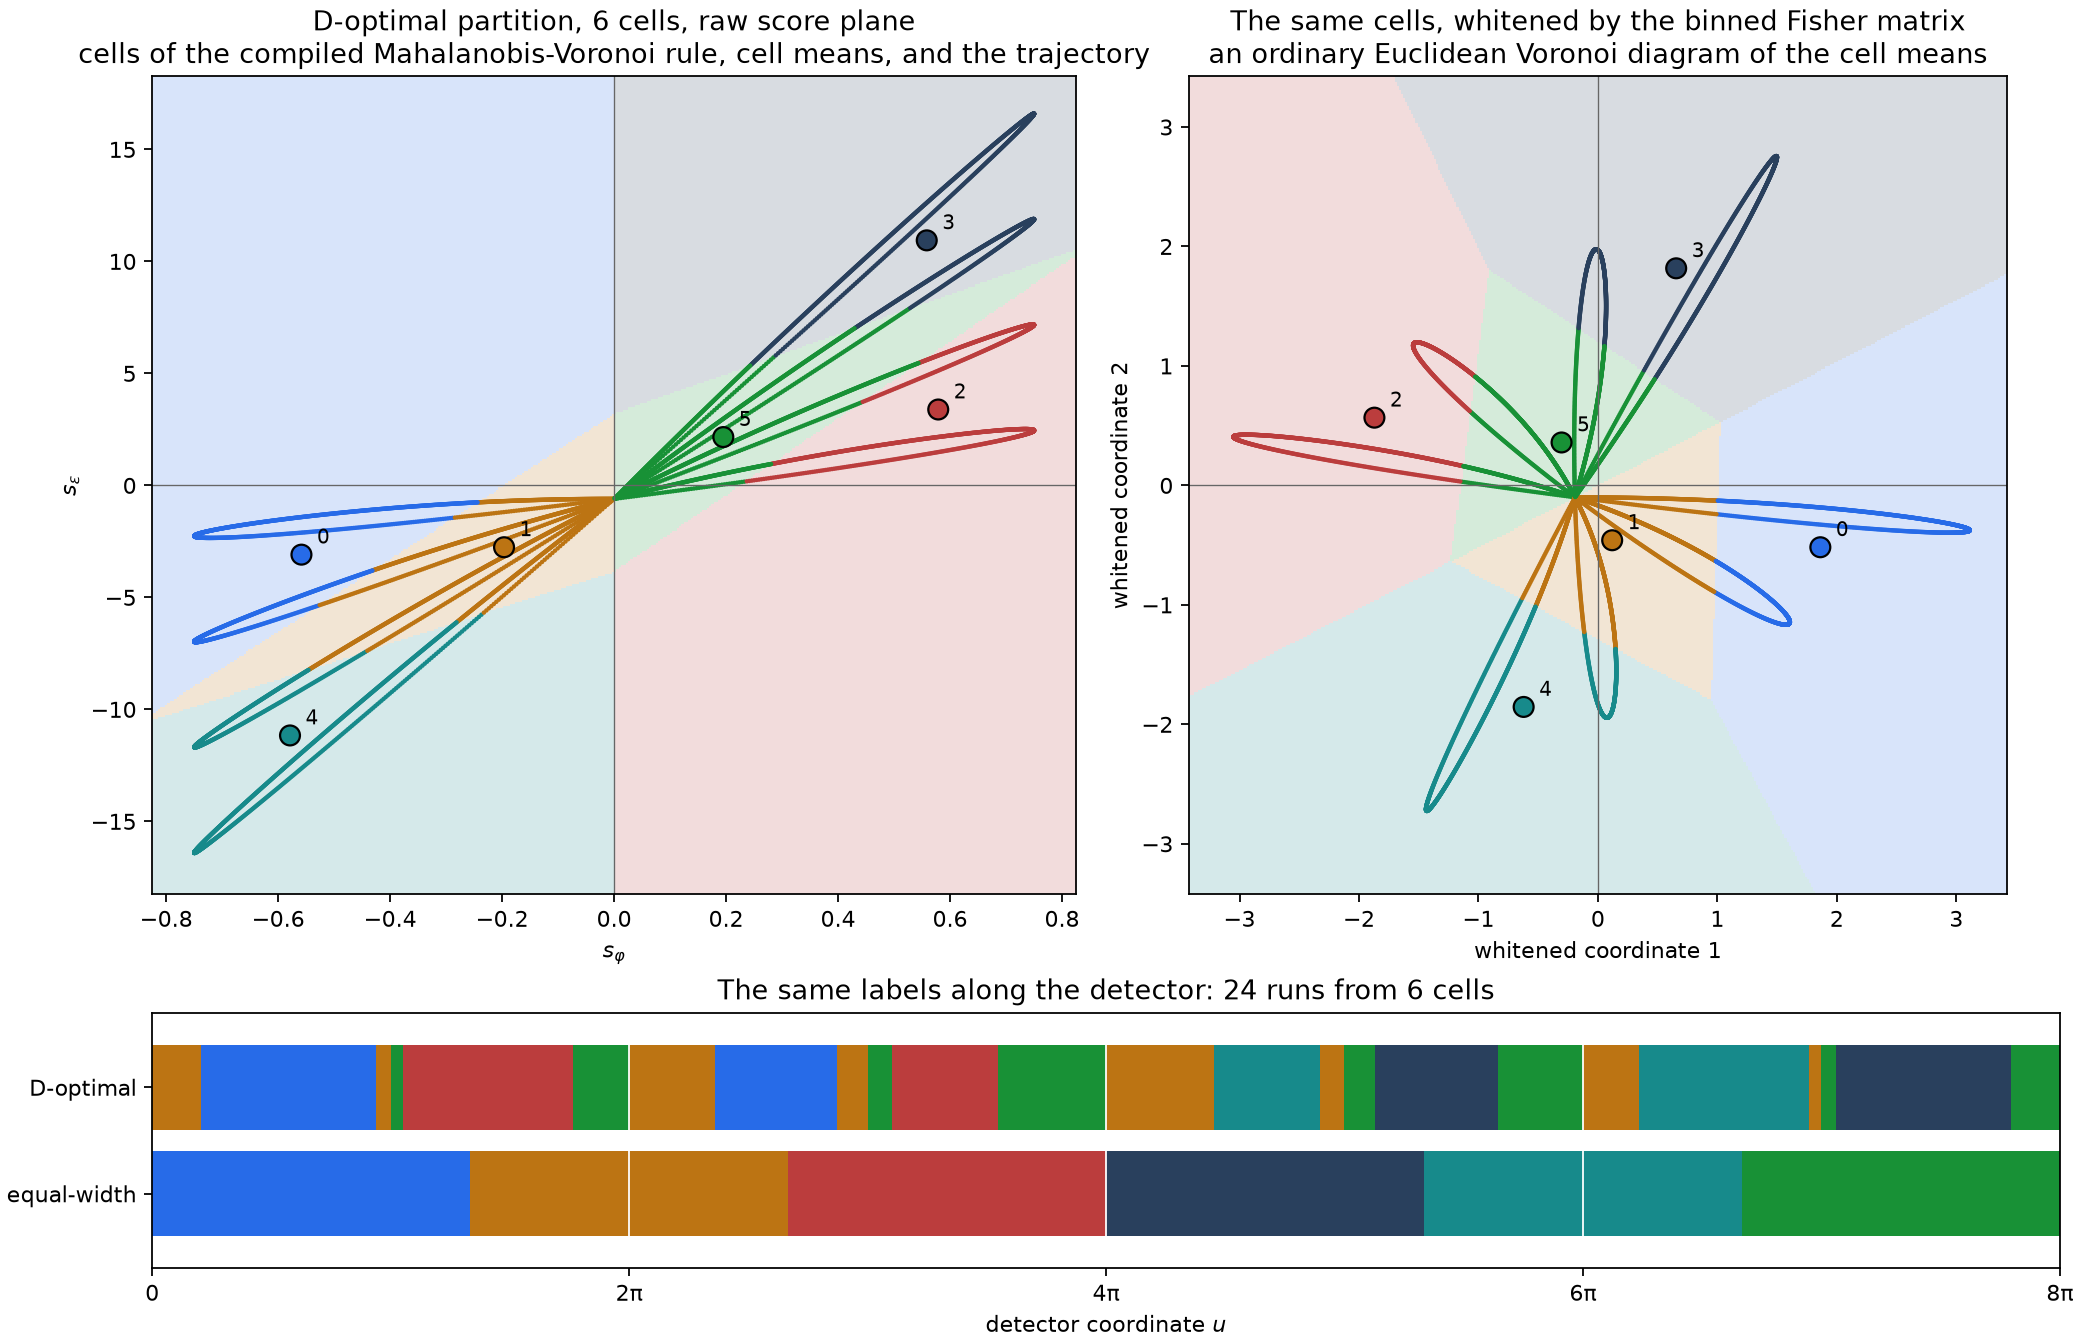
\includegraphics[width=\textwidth]{michelson-d-geometry.png}
\caption{An $\varepsilon$-stable D partition with $K=6$ of a two-parameter score: the phase of a
Michelson interferometer and a fringe-frequency error, from the library's worked example.
Top left: the compiled nearest-centroid rule in the raw score plane. Top right: after whitening
by $\Ib^{-1/2}$ the same cells are an ordinary Voronoi diagram of the cell means. Bottom: the
labels pulled back to the detector coordinate. Computed in floating point, accepting only gains
above a small tolerance $\varepsilon>0$ (Section~\ref{sec:alg}); it illustrates
Theorem~\ref{thm:main} and is not part of its proof.}
\label{fig:michelson}
\end{figure}

\subsection*{What is machine-checked}
Every result of Sections~\ref{sec:moves} and~\ref{sec:main}, the termination result of
Section~\ref{sec:alg} and the two examples of Propositions~\ref{prop:converse}
and~\ref{prop:dup} are proved in Lean~4 (v4.33.1) with Mathlib, for arbitrary dimension~$d$
(Table~\ref{tab:lean}). Most of these statements are also frozen: a specification file
(\texttt{*Spec.lean}) fixes their hypotheses, conclusion and the implication between them,
separately from the proof, and the definitions of $W_c$, $m_c$, $\mu_c$ and $\Ib$ are frozen
too. Lemma~\ref{lem:distinct}, Corollary~\ref{cor:global} and the two examples are proved but not
frozen; their statements live in the proof modules. Table~\ref{tab:lean} names the specification
of each frozen result. The build rejects warnings and unfinished proofs, and an axiom audit
admits only \texttt{propext}, \texttt{Classical.choice} and \texttt{Quot.sound}.

The Lean statements use $\det$ for stability and require positive definiteness of $\Ib$, which
for~\eqref{eq:info} is equivalent to nonsingularity. They do not cover: the identification of
$\Ib$ with the Fisher information of a statistical model; positive gain tolerances; singular or
pseudo-determinant objectives; the profiled criterion of Section~\ref{sec:nuisance}; the Lloyd
example of Section~\ref{sec:sharp} and the merged form of Proposition~\ref{prop:converse}, which
are checked in exact rational arithmetic in Python; and the software. The chaining of a terminal exchange state back to the hypotheses of
Theorem~\ref{thm:main} (Section~\ref{sec:alg}) is elementary but not mechanized.

\begin{table}[t]
\centering
\small
\begin{tabular}{@{}lll@{}}
\toprule
Result & Frozen statement & Proof declaration (module) \\
\midrule
Prop.~\ref{prop:rank2} & \texttt{RelocationSpec} & \texttt{rank\_two\_relocation} (\texttt{Relocation}) \\
Prop.~\ref{prop:detratio} & \texttt{DetGainSpec} & \texttt{det\_relocation\_gain} (\texttt{DetGain}) \\
Lemma~\ref{lem:leverage} & \texttt{LeverageSpec} & \texttt{leverage\_inequality} (\texttt{Leverage}) \\
Lemma~\ref{lem:scalar} & \texttt{ScalarExchangeSpec} & \texttt{scalarExchangeStrengthenedLowerBound} \\
Prop.~\ref{prop:gain} & \texttt{ExchangeVoronoiSpec} & \texttt{violation\_lower\_bound}, \texttt{violation\_log\_gain} \\
Lemma~\ref{lem:distinct} & --- & \texttt{centroid\_ne\_of\_stable} (\texttt{ExchangeVoronoi}) \\
Thm.~\ref{thm:main} & \texttt{ExchangeVoronoiSpec} & \texttt{exchange\_voronoi} (\texttt{ExchangeVoronoi}) \\
Cor.~\ref{cor:global} & --- & \texttt{globalOptimum\_strictVoronoi} (\texttt{Corollaries}) \\
Cor.~\ref{cor:compile} & \texttt{ClosureSpec} & \texttt{closure\_reproduces\_labels} (\texttt{Closure}) \\
Prop.~\ref{prop:merge} & \texttt{MergeSpec}, \texttt{ClosureSpec} & \texttt{merge\_invariance}, \texttt{closure\_duplicates} \\
Prop.~\ref{prop:term} & \texttt{TerminationSpec} & \texttt{terminates}, \texttt{d\_exchange\_terminates} \\
Prop.~\ref{prop:converse} (4 rows) & --- & \texttt{VoronoiConverse.*} (\texttt{Counterexamples}) \\
Prop.~\ref{prop:dup} & --- & \texttt{UnmergedDuplicates.*} (\texttt{Counterexamples}) \\
\bottomrule
\end{tabular}
\caption{Results, their frozen specifications where they have one, and their Lean proofs, all
under \texttt{research/formal/ScoreQuantFormal}. The proof of Prop.~\ref{prop:gain} is in
\texttt{ExchangeVoronoi}, that of Lemma~\ref{lem:scalar} in \texttt{ScalarExchange}.}
\label{tab:lean}
\end{table}

\section{Sharpness}\label{sec:sharp}

\subsection*{The nearest-centroid iteration can go backwards}
Theorem~\ref{thm:main} suggests a Lloyd-type iteration: compute $G=\Ib^{-1}$ and the centroids,
reassign every row to its nearest centroid in $G$, recompute, and repeat. For $k$-means, for
Bregman clustering~\cite{lloyd1982,banerjee2005}, and for the Mahalanobis reduction step of
$\min\det V$~\cite{gallegos2005}, this step never worsens the objective. For the D criterion it
can.

\begin{proposition}[non-monotone Lloyd step]\label{prop:lloyd}
For the eight rows of Table~\ref{tab:lloyd} in $\R^2$, with equal weights and $K=3$, one
reassignment to the nearest centroid in $\Ib^{-1}$ changes four labels and lowers $\log\det\Ib$
from $-3.8106$ to $-3.9472$, a loss of $0.1365$ nats. Both determinants are exact rationals,
$254982965894784407/11520000000000000000$ before and $37074006279699397/1920000000000000000$
after, and both matrices are positive definite.
\end{proposition}

\begin{table}[t]
\centering
\small
\begin{tabular}{@{}rrrcc@{}}
\toprule
row & $s_{1}$ & $s_{2}$ & label before & label after \\
\midrule
1 & $0.1116$ & $0.4427$ & 2 & 1 \\
2 & $-0.2932$ & $0.6537$ & 1 & 1 \\
3 & $-0.5995$ & $-1.2685$ & 1 & 2 \\
4 & $-0.6848$ & $-1.5456$ & 2 & 2 \\
5 & $0.4810$ & $0.9521$ & 3 & 3 \\
6 & $1.6707$ & $0.9370$ & 3 & 2 \\
7 & $0.1689$ & $1.7090$ & 3 & 1 \\
8 & $-0.8548$ & $-1.8805$ & 2 & 2 \\
\bottomrule
\end{tabular}
\caption{The Lloyd example (fixture \texttt{CE-D-LLOYD-001}, where rows and labels count from
zero); the scores are exact decimals.}
\label{tab:lloyd}
\end{table}

The reason is concavity. The step is one Lloyd step of $k$-means in the frozen metric $G$: it
lowers the within-cell distortion $\sum_iw_i\|s_i-\mu_{z_i}\|_G^2=\tr(GV(z))$, here from $13.545$
to $5.318$, and so by~\eqref{eq:pythagoras} raises $\tr(G\,I(z'))$ by $8.227$. But $\log\det$ is
concave, so
\[
\log\det I(z')\le\log\det\Ib+\tr\bigl(G(I(z')-\Ib)\bigr):
\]
the linearization bounds the gain from above, not from below. For $\min\det V$ the reduction
step reassigns in the metric $V(z)^{-1}$, which lowers $\tr(V(z)^{-1}V(z'))$, and the same tangent
inequality for the concave $\log\det V$ then gives $\log\det V(z')\le\log\det V(z)$: a
majorize--minimize step. For $\max\log\det(T-V)$ there is no such guarantee. A
batch nearest-centroid proposal must therefore be checked against the exact objective before it
is accepted.

The remaining two examples are one-dimensional, where the D criterion is $k$-means on the
scalar score. They restate facts known for $k$-means and are included only to show that the
hypotheses of Theorem~\ref{thm:main} are needed.

\subsection*{Nearest-centroid does not imply stable}

\begin{proposition}[the converse fails]\label{prop:converse}
Take $d=1$, distinct scores $(-\tfrac34,\tfrac14,\tfrac54)$, weights
$(\tfrac12,\tfrac14,\tfrac14)$, $K=2$ and labels $(1,1,2)$. The centroids are $-\tfrac5{12}$ and
$\tfrac54$, $\Ib=\tfrac{25}{48}$, and every atom is strictly nearest its own centroid. Moving the
atom at $\tfrac14$ to cell~$2$ is admissible and raises $\Ib$ to $\tfrac9{16}$.
\end{proposition}

This merged three-atom form satisfies every hypothesis of Theorem~\ref{thm:main} except
stability, and it is checked in exact rationals by \texttt{check\_numbers.py}. The Lean witness
(\texttt{VoronoiConverse}) is the same example before merging: four rows
$(-\tfrac34,-\tfrac34,\tfrac14,\tfrac54)$ of weight $\tfrac14$, with the same centroids and the
same two values of $\Ib$. Thus
\[
\text{global optimum}\ \Rightarrow\ \text{exchange stable}\ \Rightarrow\
\text{strictly nearest-centroid in }\Ib^{-1}
\]
under the hypotheses of Theorem~\ref{thm:main}, and the second implication cannot be reversed, as
for $k$-means~\cite{telgarsky2010}.

\subsection*{Unmerged duplicates}

\begin{proposition}[duplicates must be merged]\label{prop:dup}
Take $d=1$, scores $(1,1,-1)$, weights $(\tfrac14,\tfrac14,\tfrac12)$, $K=3$, each row in its own
cell. No relocation is admissible, so the labelling is exchange stable; $\Ib=1$; every hypothesis
of Theorem~\ref{thm:main} holds except distinctness of the scores, and the conclusion fails: the
first two rows are at distance $0$ from both of their centroids.
\end{proposition}

No rule that sees only the score can reproduce these labels. After merging, the theorem applies
and Proposition~\ref{prop:merge} transfers its conclusion back to the original rows.

\section{Exact exchange}\label{sec:alg}

The algorithm the theorem certifies is plain single-point exchange with exact gains. Start from a
labelling with $K$ nonempty cells and $\Ib\succ0$, for example from $k$-means on the whitened
scores or from a checked Lloyd proposal. Scan the admissible relocations, evaluate each ratio
$\rho$ by~\eqref{eq:ratio} with the cached $G$, accept a move when $\rho>1$, and update
$\Ib$, $G$ and the two centroids. Stop when no admissible move has $\rho>1$.

\begin{proposition}[strict ascent and termination]\label{prop:term}
Let $F$ be any real function of labellings, and accept a relocation only if it is admissible and
strictly increases $F$. Then every run strictly increases $F$ unless it is empty, never returns to
a labelling it has left, and has no infinite continuation; from every starting labelling some
finite run reaches a labelling at which no admissible relocation increases $F$. For
$F=\det I(\cdot)$ the terminal labelling is exchange stable in the sense of
Definition~\ref{def:move}.
\end{proposition}

\begin{proof}
Strict increase rules out cycles, and the set of labellings is finite.
\end{proof}

Admissible moves never empty a cell, and accepted moves raise $\det\Ib>0$, so a run on merged
scores started with $\Ib\succ0$ ends at a labelling that satisfies every hypothesis of
Theorem~\ref{thm:main}. Its nearest-centroid rule is then a deployable quantizer that reproduces the
training labels. Proposition~\ref{prop:term} gives no bound on the number of moves and says
nothing about global optimality; different starts can end at different stable labellings.

In floating point a solver accepts only gains above a tolerance $\varepsilon>0$, and the
guarantee weakens. If no admissible move gains more than $\varepsilon$ in $\log\det$, then by
Proposition~\ref{prop:gain} a row of a non-singleton cell $a$ that is at least as close to another
centroid $\mu_c$ satisfies
\[
q_\delta^2\ \le\ \frac{4\,(e^{\varepsilon}-1)}{\alpha\beta},\qquad q_\delta=\|\mu_a-\mu_c\|_G^2 .
\]
For a light row $\alpha\beta\approx w_i^2$, so with $w_i=1/N$ the bound reads roughly
$q_\delta\le2N\sqrt{\varepsilon}$, while Lemma~\ref{lem:leverage} already gives
$q_\delta\le1/W_a+1/W_c$, of order $K$ for balanced cells. The tolerance bound therefore says
little unless $\varepsilon\lesssim(K/N)^2$. Distinct centroids and exact reproduction of the
training labels are no longer implied, and the reference implementation checks the reproduction
rather than assuming it. This tolerance statement is not mechanized.

\section{Nuisance parameters}\label{sec:nuisance}

Often only part of $\theta$ is of interest. Write $\theta=(\psi,\lambda)$ with
$\psi\in\R^p$ of interest and $\lambda\in\R^{d-p}$ a nuisance estimated from the same labels, and
partition
\[
\Ib=\begin{pmatrix}A&B\\B\T&C\end{pmatrix},\qquad
S_\psi(z)=A-BC^{-1}B\T .
\]
The profiled information $S_\psi$ is what remains for $\psi$ after $\lambda$ is estimated, and
the $D_s$ criterion~\cite{karlin1966} maximizes
\[
F_s(z)=\log\det S_\psi(z)=\log\det\Ib-\log\det C(z)
\]
over labellings whose nuisance block $C(z)$ is nonsingular; we set $F_s(z)=-\infty$ when $C(z)$
is singular, so that $F_s$ is defined on every labelling. Exact moves still work: by
Proposition~\ref{prop:rank2} the nuisance block changes by the $\lambda$-components of the same
rank-two update, so between labellings with nonsingular blocks the gain of a move is
$\log\rho_I-\log\rho_C$, with both ratios given by~\eqref{eq:ratio}. A run started at a
labelling with $F_s>-\infty$ never accepts a move to $-\infty$, and the argument of
Proposition~\ref{prop:term}, strict increase on a finite set, applies verbatim to this
extended-real objective. (Neither statement is part of the Lean development, whose
Proposition~\ref{prop:term} is stated for real-valued~$F$.)

The gradient of $F_s$ with respect to $\Ib$ is the efficient semimetric
\[
G_s=\Ib^{-1}-J_\lambda C^{-1}J_\lambda\T=L\T S_\psi^{-1}L,\qquad L=[\,\mathrm{Id}_p,\ -BC^{-1}\,],
\]
where $J_\lambda$ selects the nuisance coordinates. It has rank $p$ and compares scores only
through the binned efficient score $e(s)=s_\psi-BC^{-1}s_\lambda$. A first-order argument
suggests that good $D_s$ partitions should be nearest-centroid in $G_s$, as D partitions are in
$\Ib^{-1}$. The finite mechanism of Section~\ref{sec:main} does not carry over: a move also
changes the nuisance block, and the change of $\log\det C$ can offset the change of
$\log\det\Ib$ in a way that the comparison in $G_s$ does not see.
The following example shows that the conclusion fails even at a global optimum.

\begin{proposition}[a non-geometric global $D_s$ optimum]\label{prop:ds}
Take the eight equal-weight scores
$(2,1),(1,7),(-4,5),(3,-8),(-2,6),(1,-8),(5,4),(6,-6)$, centred by subtracting their mean
$(\tfrac32,\tfrac18)$, with $p=1$ and $K=3$. All $966$ partitions into three nonempty cells have
a nonsingular nuisance block. The unique optimum, up to relabelling the cells, is
$z^*=(1,1,2,1,1,2,3,3)$ with $S_\psi=\tfrac{6241}{984}$; the runner-up has
$\tfrac{4232}{669}$. At $z^*$,
\[
I(z^*)=\begin{pmatrix}\tfrac{51}8&-\tfrac14\\[2pt]-\tfrac14&\tfrac{123}{64}\end{pmatrix},
\qquad e(s)=s_1+\tfrac{16}{123}\,s_2 ,
\]
and the fifth and sixth rows (centred scores $(-\tfrac72,\tfrac{47}8)$ and
$(-\tfrac12,-\tfrac{65}8)$) are strictly nearer, in $G_s$, to the centroid of the other's cell
than to their own, by margins $\tfrac{2862}{3239}$ and $\tfrac{618}{3239}$.
\end{proposition}

Since $p=1$, nearest-centroid in $G_s$ means nearest in the single coordinate $e(s)$, so the
nearest-centroid rule of $G_s$ would cut $e$ into intervals; $z^*$ is not of that form. The
example shows that no analogue of Corollary~\ref{cor:global} holds for $D_s$ with the
optimum's own efficient metric, so a finite profiled labelling cannot in general be compiled the
way a D labelling can. It does not show that $z^*$ is unrealizable by every nearest-centroid
rule: some fixed metric, or some other affine rule, under which $z^*$ is a Voronoi partition may
exist, and we have not examined this. Nor does it say anything about the population problem.

\section{A remark on estimated scores}\label{sec:estimated}

When the score is estimated, for instance from a classifier that approximates a density
ratio~\cite{brehmer2018prl,brehmer2018prd}, the theorems hold for the estimated scores $\hat s_i$,
but a retention computed from them is a surrogate: the information the labels carry is built from
the cell means of the true score. Ranking does not control the surrogate. For $s=(-2,-1,1,2)$
with equal weights and the cut at zero, the true retention is $\tfrac9{10}$; the increasing
distortions $\hat s=(-\tfrac{11}{10},-\tfrac9{10},\tfrac9{10},\tfrac{11}{10})$ and
$\hat s=(-2,-1,1,100)$ keep every label and the ordering of the scores, yet report
$\tfrac{100}{101}$ and $\tfrac{5105}{10006}\approx0.51$.

\section{Related work}\label{sec:related}

\emph{Quantization for estimation.} Fine-quantization and asymptotic analyses of detection and
estimation~\cite{poor1988,benitz1989,gubner1993} study the scalar or high-resolution regime.
Venkitasubramaniam, Tong and Swami~\cite{venkitasubramaniam2006,venkitasubramaniam2007} showed that
score-function quantizers, thresholds on the scalar score, maximize the Fisher information of a
quantized observation; Theorem~\ref{thm:main} plays the role of that statement for finite
samples, vector parameters and the determinant. Barnes, Han and \"Ozg\"ur~\cite{barnes2018,barnes2020} write the
quantized Fisher information as~\eqref{eq:info} and bound its trace; they use it for lower
bounds, not design. D\"ulek~\cite{dulek2023} shows that for exponential families some partition
of the sufficient statistic into convex polytopes maximizes the trace of the quantized Fisher
information. That is an existence result for the trace. We could read only its abstract, which
does not mention the determinant, and we found no treatment of the determinant criterion
elsewhere; our result concerns every stable partition under the determinant. Optimal quantizers for detection or mutual information are
likelihood-ratio threshold rules~\cite{tsitsiklis1993,kurkoski2014}, a different objective.

\emph{Clustering criteria and exchange.} Determinant criteria for grouping go back to Friedman and
Rubin, Marriott, and Scott and Symons~\cite{friedman1967,marriott1971,scott1971}, all for the
within-cell scatter $\det V$. Banfield and Bassill's transfer algorithm~\cite{banfield1977} contains
the update of Section~\ref{sec:moves}. Gallegos and Ritter~\cite{gallegos2005} show, for
$\min\det V$, that the Mahalanobis reduction step is monotone and that optimal clusters are
separated by Mahalanobis bisectors, results that reduce without trimming to those of
Sp\"ath~\cite{spath1985}; this is the closest structural precedent, and our
Section~\ref{sec:sharp} shows that its monotonicity does not carry over to $\max\det(T-V)$.
Hartigan's single-point method~\cite{hartigan1975,hartigan1979} and its analysis by Telgarsky and
Vattani~\cite{telgarsky2010} are the template for Theorem~\ref{thm:main} and
Proposition~\ref{prop:converse}; Slonim, Aharoni and Crammer extend Hartigan's closed-form move to
Bregman divergences~\cite{slonim2013}. For separable objectives $\sum_cW_c\phi(\mu_c)$, such as Bregman
clustering and concave impurities, Lloyd steps are monotone and optimal cells can be taken
convex~\cite{banerjee2005,burshtein1992,chou1991}; the D criterion is not separable.

\emph{Partition polytopes.} Barnes, Hoffman and Rothblum~\cite{barnes1992} prove that when an
objective is quasi-convex in the cell sums, some optimal partition has disjoint conic hulls. The
trace criterion $\sum_c|m_c|^2/W_c$ is convex in $(W_c,m_c)$ and falls under it. The
determinant does not: for $d=K=2$ and unit masses, $\det\Ib=(\det[m_1\,m_2])^2$ vanishes at
$(m_1,m_2)=(e_1,0)$ and at $(0,e_2)$ but not at their midpoint. Theorem~\ref{thm:main} is
therefore not a corollary, and it concerns every stable partition rather than the existence of a
good one.

\emph{Design of experiments.} The exchange algorithms of exact D-optimal
design~\cite{fedorov1972,mitchell1974,cook1980} use the same determinant updates to exchange design
points; there is no partition and hence no geometry. The $D_s$ criterion is
classical~\cite{karlin1966}.

\emph{Particle physics.} The score is the optimal observable for a local
measurement~\cite{atwood1992,davier1993,diehl1994}, and machine-learned score estimates are
histogrammed in practice~\cite{brehmer2017,brehmer2018prl,brehmer2018prd,brehmer2020}, with bins
chosen by hand. ThickBrick~\cite{matchev2021} trains event categorizers by a monotone Lloyd-like
iteration for discovery significance, the scalar analogue. Inference-aware and nuisance-aware
binning optimize summaries end to end against a profiled likelihood with neural
networks~\cite{decastro2019,wunsch2021,simpson2023}, and parameter fits can be optimized via
weight-derivative regression~\cite{valassi2020}. None of these gives a structural
characterization of the optimal partitions; Section~\ref{sec:nuisance} shows why one should not
expect the D characterization to survive profiling.

\section{Software and reproducibility}\label{sec:software}

The results are implemented in ScoreQuant, an MIT-licensed Python library
(\url{https://github.com/VitalyVorobyev/scorequant}). \texttt{optimize\_partition} labels a fixed
weighted sample by exact positive-gain exchange (Section~\ref{sec:alg}), merging identical score
rows by default; \texttt{compile\_quantizer} turns a terminal D labelling into the
nearest-centroid rule of Corollary~\ref{cor:compile} and refuses when the exact geometry fails at
the solver's tolerance; \texttt{fit\_quantizer} fits a reusable rule directly. Batch Lloyd
proposals are accepted only after an exact check of the objective, the safeguard
Proposition~\ref{prop:lloyd} requires. Each example of Sections~\ref{sec:sharp},
\ref{sec:nuisance} and~\ref{sec:estimated} is an exact rational fixture in
\texttt{tests/fixtures/counterexamples}, and the library names the fixture when it refuses a
request. The script
\texttt{research/paper/check\_numbers.py}, which uses only the Python standard library,
recomputes every fixture number quoted here. The Lean development is in
\texttt{research/formal} and builds with
\begin{verbatim}
cd research/formal && lake exe cache get && lake build --wfail
\end{verbatim}

\bibliographystyle{plainnat}
\bibliography{references}

\end{document}
